\title{集合与逻辑（2016--2025 高考真题）}
\author{}
\date{}
\maketitle
\noindent 本专题共 89 道题，按年份排列。每题标注原卷与原题号。

\section*{2016 年}

\begin{question}[points=5]
\textbf{来源：}2016 年 全国III卷-理科，第 1 题\par
设集合 $S=\{x|(x-2)(x-3)\ge 0\}$, $T=\{x|x>0\}$, 则 $S\cap T=$
\begin{choices}
  \item $[2,3]$
  \item $(-\infty,2]\cup[3,+\infty)$
  \item $[3,+\infty)$
  \item $(0,2]\cup[3,+\infty)$
\end{choices}
\begin{solution}
\textbf{答案：}$(0,2]\cup[3,+\infty)$

\textbf{分析：}求出 $S$ 中不等式的解集确定出 $S$, 找出 $S$ 与 $T$ 的交集即可.

\textbf{详解：}由 $S$ 中不等式解得 $x\le 2$ 或 $x\ge 3$, 即 $S=(-\infty,2]\cup[3,+\infty)$, $\because T=(0,+\infty)$, $\therefore S\cap T=(0,2]\cup[3,+\infty)$, 故选 D.
\end{solution}
\end{question}

\begin{question}[points=5]
\textbf{来源：}2016 年 全国III卷-文科，第 1 题\par
设集合 $A=\{0, 2, 4, 6, 8, 10\}$, $B=\{4, 8\}$, 则 $\complement_AB=$ ( )
\begin{choices}
  \item $\{4, 8\}$
  \item $\{0, 2, 6\}$
  \item $\{0, 2, 6, 10\}$
  \item $\{0, 2, 4, 6, 8, 10\}$
\end{choices}
\begin{solution}
\textbf{答案：}$\{0, 2, 6, 10\}$

\textbf{分析：}根据全集 $A$ 求出 $B$ 的补集即可.

\textbf{详解：}集合 $A=\{0, 2, 4, 6, 8, 10\}$, $B=\{4, 8\}$, 则 $\complement_AB=\{0, 2, 6, 10\}$. 故选 C.
\end{solution}
\end{question}

\begin{question}[points=5]
\textbf{来源：}2016 年 全国II卷-理科，第 2 题\par
已知集合$A=\{1,2,3\}$，$B=\{x|(x+1)(x-2)<0,x\in\mathbb{Z}\}$，则$A\cup B$等于（\quad）
\begin{choices}
  \item $\{1\}$
  \item $\{1,2\}$
  \item $\{0,1,2,3\}$
  \item $\{-1,0,1,2,3\}$
\end{choices}
\begin{solution}
\textbf{答案：}$\{0,1,2,3\}$

\textbf{分析：}先求出集合$A$，$B$，由此利用并集的定义能求出$A\cup B$的值．

\textbf{详解：}$B=\{x|(x+1)(x-2)<0,x\in\mathbb{Z}\}=\{0,1\}$，$A\cup B=\{0,1,2,3\}$．故选C．
\end{solution}
\end{question}

\begin{question}[points=5]
\textbf{来源：}2016 年 全国II卷-文科，第 1 题\par
已知集合$A=\{1,2,3\}$，$B=\{x|x^2<9\}$，则$A\cap B=$
\begin{choices}
  \item $\{-2,-1,0,1,2,3\}$
  \item $\{-2,-1,0,1,2\}$
  \item $\{1,2,3\}$
  \item $\{1,2\}$
\end{choices}
\begin{solution}
\textbf{答案：}$\{1,2\}$

\textbf{分析：}由$B=\{x|x^2<9\}=\{x|-3<x<3\}$，所以$A\cap B=\{1,2\}$。
\end{solution}
\end{question}

\begin{question}[points=5]
\textbf{来源：}2016 年 全国I卷-理科，第 1 题\par
设集合$A=\{x|x^2-4x+3<0\}$，$B=\{x|2x-3>0\}$，则$A\cap B=$（ ）
\begin{choices}
  \item $(-3,-\frac{3}{2})$
  \item $(-3,\frac{3}{2})$
  \item $(1,\frac{3}{2})$
  \item $(\frac{3}{2},3)$
\end{choices}
\begin{solution}
\textbf{答案：}D

\textbf{分析：}解不等式求出集合$A$，$B$，结合交集的定义，可得答案．

\textbf{详解：}解：因为集合$A=\{x|x^2-4x+3<0\}=(1,3)$，$B=\{x|2x-3>0\}=(\frac{3}{2},+\infty)$，所以$A\cap B=(\frac{3}{2},3)$，故选：D．
\end{solution}
\end{question}

\begin{question}[points=5]
\textbf{来源：}2016 年 全国I卷-文科，第 1 题\par
设集合$A=\{1,3,5,7\}$，$B=\{x|2\le x\le5\}$，则$A\cap B=$
\begin{choices}
  \item $\{1,3\}$
  \item $\{3,5\}$
  \item $\{5,7\}$
  \item $\{1,7\}$
\end{choices}
\begin{solution}
\textbf{答案：}$\{3,5\}$

\textbf{分析：}直接利用交集的运算法则化简求解即可。

\textbf{详解：}集合$A=\{1,3,5,7\}$，$B=\{x|2\le x\le5\}$，则$A\cap B=\{3,5\}$。故选：$B$。
\end{solution}
\end{question}

\section*{2017 年}

\begin{question}[points=5]
\textbf{来源：}2017 年 全国III卷-理科，第 1 题\par
已知集合$A=\{(x,y)|x^2+y^2=1\}$，$B=\{(x,y)|y=x\}$，则$A\cap B$中元素的个数为（ ）
\begin{choices}
  \item $3$
  \item $2$
  \item $1$
  \item $0$
\end{choices}
\begin{solution}
\textbf{答案：}$B$

\textbf{分析：}解不等式组求出元素的个数即可。

\textbf{详解：}由$\begin{cases} x^2+y^2=1 \\ y=x \end{cases}$，解得：$\begin{cases} x=\frac{\sqrt{2}}{2} \\ y=\frac{\sqrt{2}}{2} \end{cases}$或$\begin{cases} x=-\frac{\sqrt{2}}{2} \\ y=-\frac{\sqrt{2}}{2} \end{cases}$，所以$A\cap B$的元素的个数是2个。故选B。
\end{solution}
\end{question}

\begin{question}[points=5]
\textbf{来源：}2017 年 全国III卷-文科，第 1 题\par
已知集合$A=\{1,2,3,4\}$，$B=\{2,4,6,8\}$，则$A\cap B$中元素的个数为（    ）
\begin{choices}
  \item A．$1$
  \item B．$2$
  \item C．$3$
  \item D．$4$
\end{choices}
\begin{solution}
\textbf{答案：}B

\textbf{分析：}利用交集定义先求出$A\cap B$，由此能求出$A\cap B$中元素的个数。

\textbf{详解：}集合$A=\{1,2,3,4\}$，$B=\{2,4,6,8\}$，则$A\cap B=\{2,4\}$，故个数为$2$。
\end{solution}
\end{question}

\begin{question}[points=5]
\textbf{来源：}2017 年 全国II卷-理科，第 2 题\par
设集合 $A=\{1,2,4\}$，$B=\{x|x^2-4x+m=0\}$．若 $A\cap B=\{1\}$，则 $B=$（   ）
\begin{choices}
  \item $\{1,-3\}$
  \item $\{1,0\}$
  \item $\{1,3\}$
  \item $\{1,5\}$
\end{choices}
\begin{solution}
\textbf{答案：}$C$

\textbf{分析：}由交集的定义可得 $1\in A$ 且 $1\in B$，代入二次方程，求得 $m$，再解二次方程可得集合 $B$。

\textbf{详解：}集合 $A=\{1,2,4\}$，$B=\{x|x^2-4x+m=0\}$．若 $A\cap B=\{1\}$，则 $1\in A$ 且 $1\in B$，可得 $1-4+m=0$，解得 $m=3$，即有 $B=\{x|x^2-4x+3=0\}=\{1,3\}$．故选：$C$。
\end{solution}
\end{question}

\begin{question}[points=5]
\textbf{来源：}2017 年 全国II卷-文科，第 1 题\par
设集合 $A=\{1,2,3\}$, $B=\{2,3,4\}$, 则 $A\cup B=$
\begin{choices}
  \item $\{1,2,3,4\}$
  \item $\{1,2,3\}$
  \item $\{2,3,4\}$
  \item $\{1,3,4\}$
\end{choices}
\begin{solution}
\textbf{答案：}$\{1,2,3,4\}$

\textbf{分析：}集合 $A=\{1,2,3\}$, $B=\{2,3,4\}$, 求 $A\cup B$, 可用并集的定义直接求出两集合的并集.

\textbf{详解：}$\because A=\{1,2,3\}$, $B=\{2,3,4\}$, $\therefore A\cup B=\{1,2,3,4\}$. 故选A.
\end{solution}
\end{question}

\begin{question}[points=5]
\textbf{来源：}2017 年 全国I卷-理科，第 1 题\par
已知集合 $A=\{x|x<1\}$，$B=\{x|3^x<1\}$，则（ ）
\begin{choices}
  \item $A\cap B=\{x|x<0\}$
  \item $A\cup B=\mathbb{R}$
  \item $A\cup B=\{x|x>1\}$
  \item $A\cap B=\varnothing$
\end{choices}
\begin{solution}
\textbf{答案：}A

\textbf{分析：}先分别求出集合 $A$ 和 $B$，再求出 $A\cap B$ 和 $A\cup B$，由此能求出结果．

\textbf{详解：}因为集合 $A=\{x|x<1\}$，$B=\{x|3^x<1\}=\{x|x<0\}$，所以$A\cap B=\{x|x<0\}$，故 A 正确，D 错误；$A\cup B=\{x|x<1\}$，故 B 和 C 都错误．故选：A．
\end{solution}
\end{question}

\begin{question}[points=5]
\textbf{来源：}2017 年 全国I卷-文科，第 1 题\par
已知集合$A=\{x|x<2\}$，$B=\{x|3-2x>0\}$，则（        ）
\begin{choices}
  \item $A\cap B=\{x|x<\frac{3}{2}\}$
  \item $A\cap B=\varnothing$
  \item $A\cup B=\{x|x<\frac{3}{2}\}$
  \item $A\cup B=\mathbb{R}$
\end{choices}
\begin{solution}
\textbf{答案：}A

\textbf{分析：}解不等式求出集合$B$，结合集合交集和并集的定义，可得结论。

\textbf{详解：}解：$\because$集合$A=\{x|x<2\}$，$B=\{x|3-2x>0\}=\{x|x<\frac{3}{2}\}$，$\therefore A\cap B=\{x|x<\frac{3}{2}\}$，故A正确，B错误；$A\cup B=\{x|x<2\}$，故C，D错误；故选：A。
\end{solution}
\end{question}

\section*{2018 年}

\begin{question}[points=5]
\textbf{来源：}2018 年 全国III卷-理科，第 1 题\par
已知集合$A=\{x|x-1\geq 0\}$，$B=\{0,1,2\}$，则$A\cap B=$（ ）
\begin{choices}
  \item $\{0\}$
  \item $\{1\}$
  \item $\{1,2\}$
  \item $\{0,1,2\}$
\end{choices}
\begin{solution}
\textbf{答案：}C

\textbf{分析：}求解不等式化简集合$A$，再由交集的运算性质得答案．

\textbf{详解：}$\because A=\{x|x-1\geq 0\}=\{x|x\geq 1\}$，$B=\{0,1,2\}$，$\therefore A\cap B=\{x|x\geq 1\}\cap\{0,1,2\}=\{1,2\}$．
\end{solution}
\end{question}

\begin{question}[points=5]
\textbf{来源：}2018 年 全国III卷-文科，第 1 题\par
已知集合 $A=\{x|x-1\ge 0\}$，$B=\{0,1,2\}$，则 $A\cap B=$
\begin{choices}
  \item $\{0\}$
  \item $\{1\}$
  \item $\{1,2\}$
  \item $\{0,1,2\}$
\end{choices}
\begin{solution}
\textbf{答案：}C

\textbf{分析：}求解不等式化简集合 $A$，再由交集的运算性质得答案．

\textbf{详解：}$\because A=\{x|x-1\ge 0\}=\{x|x\ge 1\}$，$B=\{0,1,2\}$，$\therefore A\cap B=\{x|x\ge 1\}\cap\{0,1,2\}=\{1,2\}$．故选：C．
\end{solution}
\end{question}

\begin{question}[points=5]
\textbf{来源：}2018 年 全国II卷-理科，第 2 题\par
已知集合$A=\{(x,y)|x^2+y^2\le 3, x\in \mathbb{Z}, y\in \mathbb{Z}\}$，则$A$中元素的个数为（     ）
\begin{choices}
  \item $9$
  \item $8$
  \item $5$
  \item $4$
\end{choices}
\begin{solution}
\textbf{答案：}A

\textbf{分析：}分别令$x=-1,0,1$，进行求解即可．

\textbf{详解：}当$x=-1$时，$y^2\le 2$，得$y=-1,0,1$；当$x=0$时，$y^2\le 3$，得$y=-1,0,1$；当$x=1$时，$y^2\le 2$，得$y=-1,0,1$．即集合$A$中元素有$9$个，故选A．
\end{solution}
\end{question}

\begin{question}[points=5]
\textbf{来源：}2018 年 全国II卷-文科，第 2 题\par
已知集合 $A=\{1,3,5,7\}$，$B=\{2,3,4,5\}$，则 $A\cap B=$（ ）
\begin{choices}
  \item $\{3\}$
  \item $\{5\}$
  \item $\{3,5\}$
  \item $\{1,2,3,4,5,7\}$
\end{choices}
\begin{solution}
\textbf{答案：}$\{3,5\}$

\textbf{分析：}利用交集定义直接求解。

\textbf{详解：}因为集合 $A=\{1,3,5,7\}$，$B=\{2,3,4,5\}$，所以$A\cap B=\{3,5\}$。故选：C。
\end{solution}
\end{question}

\begin{question}[points=5]
\textbf{来源：}2018 年 全国I卷-理科，第 2 题\par
已知集合$A=\{x|x^2-x-2>0\}$，则$\complement_RA=$（    ）
\begin{choices}
  \item $\{x|-1<x<2\}$
  \item $\{x|-1\leq x\leq2\}$
  \item $\{x|x<-1\}\cup\{x|x>2\}$
  \item $\{x|x\leq-1\}\cup\{x|x\geq2\}$
\end{choices}
\begin{solution}
\textbf{答案：}B

\textbf{分析：}通过求解不等式，得到集合$A$，然后求解补集即可。

\textbf{详解：}集合$A=\{x|x^2-x-2>0\}$，可得$A=\{x|x<-1\text{或}x>2\}$，则$\complement_RA=\{x|-1\leq x\leq2\}$。故选B。
\end{solution}
\end{question}

\begin{question}[points=5]
\textbf{来源：}2018 年 全国I卷-文科，第 1 题\par
已知集合 $A=\{0,2\}$，$B=\{-2,-1,0,1,2\}$，则 $A\cap B=$
\begin{choices}
  \item $\{0,2\}$
  \item $\{1,2\}$
  \item $\{0\}$
  \item $\{-2,-1,0,1,2\}$
\end{choices}
\begin{solution}
\textbf{答案：}$\{0,2\}$

\textbf{分析：}直接利用集合的交集的运算法则求解即可。

\textbf{详解：}集合 $A=\{0,2\}$，$B=\{-2,-1,0,1,2\}$，则 $A\cap B=\{0,2\}$。故选：$A$。
\end{solution}
\end{question}

\section*{2019 年}

\begin{question}[points=5]
\textbf{来源：}2019 年 全国III卷-理科，第 1 题\par
已知集合 $A = \{-1, 0, 1, 2\}$，$B = \{x \mid x^2 \le 1\}$，则 $A \cap B =$
\begin{choices}
  \item $\{-1,0,1\}$
  \item $\{0,1\}$
  \item $\{-1,1\}$
  \item $\{0,1,2\}$
\end{choices}
\begin{solution}
\textbf{答案：}A

\textbf{分析：}先求出集合 $B$，再求交集。

\textbf{详解：}由题意得 $B = \{x \mid -1 \le x \le 1\}$，则 $A \cap B = \{-1,0,1\}$。故选 A。
\end{solution}
\end{question}

\begin{question}[points=5]
\textbf{来源：}2019 年 全国III卷-文科，第 1 题\par
已知集合$A=\{-1,0,1,2\}$，$B=\{x|x^2\le 1\}$，则$A\cap B=$
\begin{choices}
  \item $\{-1,0,1\}$
  \item $\{0,1\}$
  \item $\{-1,1\}$
  \item $\{0,1,2\}$
\end{choices}
\begin{solution}
\textbf{答案：}A

\textbf{分析：}先求出集合$B$再求出交集。

\textbf{详解：}由题意得，$B=\{x|-1\le x\le 1\}$，则$A\cap B=\{-1,0,1\}$。故选A。
\end{solution}
\end{question}

\begin{question}[points=5]
\textbf{来源：}2019 年 全国III卷-文科，第 11 题；次专题：一元二次函数、方程和不等式\par
记不等式组$\begin{cases} x+y\le 6 \\ 2x-y\ge 0 \end{cases}$表示的平面区域为D。命题$p:\exists(x,y)\in D,2x+y\le 9$；命题$q:\forall(x,y)\in D,2x+y\le 12$。下面给出了四个命题：①$p\lor q$；②$\neg p\lor q$；③$p\land \neg q$；④$\neg p\land \neg q$。这四个命题中，所有真命题的编号是

\begin{center}
  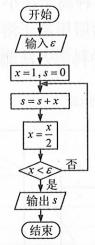
\includegraphics[width=.42\linewidth]{assets/asset-021-01.jpg}
\end{center}
\begin{choices}
  \item ①③
  \item ①②
  \item ②③
  \item ③④
\end{choices}
\begin{solution}
\textbf{答案：}A

\textbf{分析：}根据题意可画出平面区域再结合命题可判断出真命题。

\textbf{详解：}如图，平面区域D为阴影部分，由$\begin{cases} y=2x \\ x+y=6 \end{cases}$得$\begin{cases} x=2 \\ y=4 \end{cases}$，即A(2,4)，直线$2x+y=9$与直线$2x+y=12$均过区域D，则$p$真$q$假，有$\neg p$假$\neg q$真，所以①③真②④假。故选A。
\end{solution}
\end{question}

\begin{question}[points=5]
\textbf{来源：}2019 年 全国II卷-理科，第 1 题\par
设集合 $A=\{x|x^2-5x+6>0\}$，$B=\{x|x-1<0\}$，则 $A\cap B$=
\begin{choices}
  \item $(-\infty,1)$
  \item $(-2,1)$
  \item $(-3,-1)$
  \item $(3,+\infty)$
\end{choices}
\begin{solution}
\textbf{答案：}$A$

\textbf{分析：}本题考查集合的交集和一元二次不等式的解法，渗透了数学运算素养．采取数轴法，利用数形结合的思想解题．

\textbf{详解：}由题意得，$A=\{x|x<2 \text{ 或 } x>3\}$，$B=\{x|x<1\}$，则 $A\cap B=\{x|x<1\}$．故选 $A$．
\end{solution}
\end{question}

\begin{question}[points=5]
\textbf{来源：}2019 年 全国II卷-文科，第 1 题\par
已知集合 $A=\{x\mid x>-1\}$，$B=\{x\mid x<2\}$，则 $A\cap B=$
\begin{choices}
  \item $(-1,+\infty)$
  \item $(-\infty,2)$
  \item $(-1,2)$
  \item $\varnothing$
\end{choices}
\begin{solution}
\textbf{答案：}$C$

\textbf{分析：}本题借助于数轴，根据交集的定义可得．

\textbf{详解：}由题知，$A\cap B=(-1,2)$，故选 $C$．
\end{solution}
\end{question}

\begin{question}[points=5]
\textbf{来源：}2019 年 全国II卷-文科，第 5 题\par
在“一带一路”知识测验后，甲、乙、丙三人对成绩进行预测．

甲：我的成绩比乙高．

乙：丙的成绩比我和甲的都高．

丙：我的成绩比乙高．

成绩公布后，三人成绩互不相同且只有一个人预测正确，那么三人按成绩由高到低的次序为
\begin{choices}
  \item 甲、乙、丙
  \item 乙、甲、丙
  \item 丙、乙、甲
  \item 甲、丙、乙
\end{choices}
\begin{solution}
\textbf{答案：}$A$

\textbf{分析：}利用逐一验证的方法进行求解．

\textbf{详解：}若甲预测正确，则乙、丙预测错误，则甲比乙成绩高，丙比乙成绩低，故 $3$ 人成绩由高到低依次为甲，乙，丙；若乙预测正确，则丙预测也正确，不符合题意；若丙预测正确，则甲必预测错误，丙比乙的成绩高，乙比甲成绩高，即丙比甲、乙成绩都高，即乙预测正确，不符合题意，故选 $A$．
\end{solution}
\end{question}

\begin{question}[points=5]
\textbf{来源：}2019 年 全国I卷-理科，第 1 题\par
已知集合 $M = \{x \mid -4 < x < 2\}$, $N = \{x \mid x^2 - x - 6 < 0\}$, 则 $M \cap N =$
\begin{choices}
  \item $\{x \mid -4 < x < 3\}$
  \item $\{x \mid -4 < x < -2\}$
  \item $\{x \mid -2 < x < 2\}$
  \item $\{x \mid 2 < x < 3\}$
\end{choices}
\begin{solution}
\textbf{答案：}$C$

\textbf{分析：}本题考查集合的交集和一元二次不等式的解法，渗透了数学运算素养．采取数轴法，利用数形结合的思想解题．

\textbf{详解：}由题意得，$M = \{x \mid -4 < x < 2\}$, $N = \{x \mid -2 < x < 3\}$, 则 $M \cap N = \{x \mid -2 < x < 2\}$．故选 $C$．
\end{solution}
\end{question}

\begin{question}[points=5]
\textbf{来源：}2019 年 全国I卷-文科，第 2 题\par
已知集合 $U = \{1,2,3,4,5,6,7\}$，$A = \{2,3,4,5\}$，$B = \{2,3,6,7\}$，则 $B \cap \complement_U A =$
\begin{choices}
  \item $\{1,6\}$
  \item $\{1,7\}$
  \item $\{6,7\}$
  \item $\{1,6,7\}$
\end{choices}
\begin{solution}
\textbf{答案：}C

\textbf{分析：}先求 $\complement_U A$，再求 $B \cap \complement_U A$。

\textbf{详解：}由已知得 $\complement_U A = \{1,6,7\}$，所以 $B \cap \complement_U A = \{6,7\}$，故选 C。
\end{solution}
\end{question}

\section*{2020 年}

\begin{question}[points=5]
\textbf{来源：}2020 年 全国III卷-理科，第 1 题\par
已知集合 $A=\{(x,y)\mid x,y\in\mathbb{N}^*,\ y\ge x\}$，$B=\{(x,y)\mid x+y=8\}$，则 $A\cap B$ 中元素的个数为
\begin{choices}
  \item $2$
  \item $3$
  \item $4$
  \item $6$
\end{choices}
\begin{solution}
\textbf{答案：}$C$

\textbf{分析：}采用列举法列举出 $A\cap B$ 中元素即可。

\textbf{详解：}由题意，$A\cap B$ 中的元素满足 $\begin{cases} y\ge x \\ x+y=8 \end{cases}$，且 $x,y\in\mathbb{N}^*$，由 $x+y=8\ge 2x$，得 $x\le 4$，所以满足 $x+y=8$ 的有 $(1,7),(2,6),(3,5),(4,4)$，故 $A\cap B$ 中元素的个数为 $4$。故选 $C$。
\end{solution}
\end{question}

\begin{question}[points=5]
\textbf{来源：}2020 年 全国III卷-文科，第 1 题\par
已知集合 $A=\{1,2,3,5,7,11\}$，$B=\{x|3<x<15\}$，则 $A\cap B$ 中元素的个数为
\begin{choices}
  \item $2$
  \item $3$
  \item $4$
  \item $5$
\end{choices}
\begin{solution}
\textbf{答案：}B

\textbf{分析：}采用列举法列举出 $A\cap B$ 中元素的即可.

\textbf{详解：}由题意，$A\cap B=\{5,7,11\}$，故 $A\cap B$ 中元素的个数为3. 故选：B.
\end{solution}
\end{question}

\begin{question}[points=5]
\textbf{来源：}2020 年 全国II卷-理科，第 1 题\par
已知集合 $U=\{-2,-1,0,1,2,3\}$，$A=\{-1,0,1\}$，$B=\{1,2\}$，则 $\complement_U(A\cup B)=$ （ ）
\begin{choices}
  \item $\{-2,3\}$
  \item $\{-2,2,3\}$
  \item $\{-2,-1,0,3\}$
  \item $\{-2,-1,0,2,3\}$
\end{choices}
\begin{solution}
\textbf{答案：}$\{-2,3\}$

\textbf{分析：}首先进行并集运算，然后计算补集即可.

\textbf{详解：}由题意可得：$A\cup B=\{-1,0,1,2\}$，则 $\complement_U(A\cup B)=\{-2,3\}$.
\end{solution}
\end{question}

\begin{question}[points=5]
\textbf{来源：}2020 年 全国II卷-理科，第 16 题；次专题：立体几何\par
设有下列四个命题：

$p_1$：两两相交且不过同一点的三条直线必在同一平面内.

$p_2$：过空间中任意三点有且仅有一个平面.

$p_3$：若空间两条直线不相交，则这两条直线平行.

$p_4$：若直线$l\subset$平面$\alpha$，直线$m\perp$平面$\alpha$，则$m\perp l$.

则下述命题中所有真命题的序号是.

①$p_1\land p_4$ ②$p_1\land p_2$ ③$\lnot p_2\lor p_3$ ④$\lnot p_3\lor\lnot p_4$
\fillin[{$①③④$}]
\begin{solution}
\textbf{答案：}$①③④$

\textbf{分析：}利用两交线直线确定一个平面可判断命题$p_1$的真假；利用三点共线可判断命题$p_2$的真假；利用异面直线可判断命题$p_3$的真假，利用线面垂直的定义可判断命题$p_4$的真假.再利用复合命题的真假可得出结论.

\textbf{详解：}对于命题$p_1$，可设$l_1$与$l_2$相交，这两条直线确定的平面为$\alpha$；若$l_3$与$l_1$相交，则交点$A$在平面$\alpha$内，同理，$l_3$与$l_2$的交点$B$也在平面$\alpha$内，所以$AB\subset\alpha$，即$l_3\subset\alpha$，命题$p_1$为真命题；对于命题$p_2$，若三点共线，则过这三个点的平面有无数个，命题$p_2$为假命题；对于命题$p_3$，空间中两条直线相交、平行或异面，命题$p_3$为假命题；对于命题$p_4$，若直线$m\perp$平面$\alpha$，则$m$垂直于平面$\alpha$内所有直线，$\because$直线$l\subset$平面$\alpha$，$\therefore$直线$m\perp$直线$l$，命题$p_4$为真命题.综上可知，$p_1\land p_4$为真命题，$p_1\land p_2$为假命题，$\lnot p_2\lor p_3$为真命题，$\lnot p_3\lor\lnot p_4$为真命题.故答案为：①③④.
\end{solution}
\end{question}

\begin{question}[points=5]
\textbf{来源：}2020 年 全国II卷-文科，第 1 题\par
已知集合 $A=\{x||x|<3, x \in Z\}$，$B=\{x||x|>1, x \in Z\}$，则 $A \cap B=$（ ）
\begin{choices}
  \item $\varnothing$
  \item $\{-3, -2, 2, 3\}$
  \item $\{-2, 0, 2\}$
  \item $\{-2, 2\}$
\end{choices}
\begin{solution}
\textbf{答案：}D

\textbf{分析：}解绝对值不等式化简集合 $A, B$ 的表示，再根据集合交集的定义进行求解即可。

\textbf{详解：}因为 $A=\{x||x|<3, x \in Z\}=\{-2, -1, 0, 1, 2\}$，$B=\{x||x|>1, x \in Z\}=\{x|x>1 \text{ 或 } x<-1, x \in Z\}$，所以 $A \cap B=\{2, -2\}$。
故选：D。
\end{solution}
\end{question}

\begin{question}[points=5]
\textbf{来源：}2020 年 全国II卷-文科，第 16 题；次专题：立体几何\par
设有下列四个命题：

$p_1$：两两相交且不过同一点的三条直线必在同一平面内。

$p_2$：过空间中任意三点有且仅有一个平面。

$p_3$：若空间两条直线不相交，则这两条直线平行。

$p_4$：若直线 $l \subset$ 平面 $\alpha$，直线 $m\perp$ 平面 $\alpha$，则 $m\perp l$。

则下述命题中所有真命题的序号是。

① $p_1 \land p_4$ ② $p_1 \land p_2$ ③ $\lnot p_2 \lor p_3$ ④ $\lnot p_3 \lor \lnot p_4$
\fillin[{$①③④$}]
\begin{solution}
\textbf{答案：}$①③④$

\textbf{分析：}利用两相交直线确定一个平面可判断命题 $p_1$ 的真假；利用三点共线可判断命题 $p_2$ 的真假；利用异面直线可判断命题 $p_3$ 的真假；利用线面垂直的定义可判断命题 $p_4$ 的真假。再利用复合命题的真假可得出结论。

\textbf{详解：}对于命题 $p_1$，可设 $l_1$ 与 $l_2$ 相交，这两条直线确定的平面为 $\alpha$；若 $l_3$ 与 $l_1$ 相交，则交点 $A$ 在平面 $\alpha$ 内，同理，$l_3$ 与 $l_2$ 的交点 $B$ 也在平面 $\alpha$ 内，所以 $AB\subset \alpha$，即 $l_3\subset \alpha$，命题 $p_1$ 为真命题。
对于命题 $p_2$，若三点共线，则过这三个点的平面有无数个，命题 $p_2$ 为假命题。
对于命题 $p_3$，空间中两条直线相交、平行或异面，命题 $p_3$ 为假命题。
对于命题 $p_4$，若直线 $m\perp$ 平面 $\alpha$，则 $m$ 垂直于平面 $\alpha$ 内所有直线，$\because$ 直线 $l\subset$ 平面 $\alpha$，$\therefore$ 直线 $m\perp$ 直线 $l$，命题 $p_4$ 为真命题。
综上可知，$p_1\land p_4$ 为真命题，$p_1\land p_2$ 为假命题，$\lnot p_2\lor p_3$ 为真命题，$\lnot p_3\lor \lnot p_4$ 为真命题。
故答案为：①③④。
\end{solution}
\end{question}

\begin{question}[points=5]
\textbf{来源：}2020 年 全国I卷-理科，第 2 题；次专题：一元二次函数、方程和不等式\par
设集合$A=\{x|x^2-4\leq 0\}$，$B=\{x|2x+a\leq 0\}$，且$A\cap B=\{x|-2\leq x\leq 1\}$，则$a=$
\begin{choices}
  \item $-4$
  \item $-2$
  \item $2$
  \item $4$
\end{choices}
\begin{solution}
\textbf{答案：}B

\textbf{详解：}由$x^2-4\leq 0$得$A=\{x|-2\leq x\leq 2\}$，由$2x+a\leq 0$得$B=\{x|x\leq -\frac{a}{2}\}$。因为$A\cap B=\{x|-2\leq x\leq 1\}$，所以$-\frac{a}{2}=1$，解得$a=-2$。
\end{solution}
\end{question}

\begin{question}[points=5]
\textbf{来源：}2020 年 全国I卷-文科，第 1 题\par
已知集合 $A = \{x \mid x^2 - 3x - 4 < 0\}$, $B = \{-4, 1, 3, 5\}$, 则 $A \cap B =$
\begin{choices}
  \item $\{-4, 1\}$
  \item $\{1, 5\}$
  \item $\{3, 5\}$
  \item $\{1, 3\}$
\end{choices}
\begin{solution}
\textbf{答案：}$\{1, 3\}$

\textbf{分析：}首先解一元二次不等式求得集合 $A$, 之后利用交集中元素的特征求得 $A \cap B$.

\textbf{详解：}由 $x^2 - 3x - 4 < 0$ 解得 $-1 < x < 4$, 所以 $A = \{x \mid -1 < x < 4\}$, 又因为 $B = \{-4, 1, 3, 5\}$, 所以 $A \cap B = \{1, 3\}$.
\end{solution}
\end{question}

\section*{2021 年}

\begin{question}[points=4]
\textbf{来源：}2021 年 北京卷，第 1 题\par
已知集合 $A=\{x\mid -1<x<1\}$, $B=\{x\mid 0\leq x\leq 2\}$, 则 $A\cup B=$ （ ）
\begin{choices}
  \item $(-1,2)$
  \item $(-1,2]$
  \item $[0,1)$
  \item $[0,1]$
\end{choices}
\begin{solution}
\textbf{答案：}B

\textbf{分析：}结合题意利用并集的定义计算即可.

\textbf{详解：}由题意可得 $A\cup B=\{x\mid -1<x\leq 2\}$, 即 $A\cup B=(-1,2]$.
\end{solution}
\end{question}

\begin{question}[points=4]
\textbf{来源：}2021 年 北京卷，第 3 题；次专题：函数\par
已知 $f(x)$ 是定义在 $[0,1]$ 上的函数, 那么“函数 $f(x)$ 在 $[0,1]$ 上单调递增”是“函数 $f(x)$ 在 $[0,1]$ 上的最大值为 $f(1)$”的（ ）
\begin{choices}
  \item 充分而不必要条件
  \item 必要而不充分条件
  \item 充分必要条件
  \item 既不充分也不必要条件
\end{choices}
\begin{solution}
\textbf{答案：}A

\textbf{分析：}利用两者之间的推出关系可判断两者之间的条件关系.

\textbf{详解：}若函数 $f(x)$ 在 $[0,1]$ 上单调递增, 则 $f(x)$ 在 $[0,1]$ 上的最大值为 $f(1)$; 若 $f(x)$ 在 $[0,1]$ 上的最大值为 $f(1)$, 比如 $f(x)=\left(x-\frac{1}{3}\right)^2$, 但 $f(x)=\left(x-\frac{1}{3}\right)^2$ 在 $\left[0,\frac{1}{3}\right]$ 为减函数, 在 $\left[\frac{1}{3},1\right]$ 为增函数, 故 $f(x)$ 在 $[0,1]$ 上的最大值为 $f(1)$ 推不出 $f(x)$ 在 $[0,1]$ 上单调递增, 故“函数 $f(x)$ 在 $[0,1]$ 上单调递增”是“$f(x)$ 在 $[0,1]$ 上的最大值为 $f(1)$”的充分不必要条件.
\end{solution}
\end{question}

\begin{question}[points=5]
\textbf{来源：}2021 年 全国甲卷-理科，第 1 题\par
设集合 $M = \{x \mid 0 < x < 4\}$, $N = \left\{x \mid \frac{1}{3} \le x \le 5\right\}$, 则 $M \cap N =$ ( )
\begin{choices}
  \item $\left\{x \mid 0 < x \le \frac{1}{3}\right\}$
  \item $\left\{x \mid \frac{1}{3} \le x < 4\right\}$
  \item $\{x \mid 4 \le x < 5\}$
  \item $\{x \mid 0 < x \le 5\}$
\end{choices}
\begin{solution}
\textbf{答案：}B

\textbf{分析：}根据交集定义运算即可

\textbf{详解：}$M = \{x \mid 0 < x < 4\}$, $N = \left\{x \mid \frac{1}{3} \le x \le 5\right\}$, 则 $M \cap N = \left\{x \mid \frac{1}{3} \le x < 4\right\}$．
\end{solution}
\end{question}

\begin{question}[points=5]
\textbf{来源：}2021 年 全国甲卷-文科，第 1 题\par
设集合 $M = \{1,3,5,7,9\}$, $N = \{x \mid 2x > 7\}$, 则 $M \cap N =$ ( )
\begin{choices}
  \item $\{7,9\}$
  \item $\{5,7,9\}$
  \item $\{3,5,7,9\}$
  \item $\{1,3,5,7,9\}$
\end{choices}
\begin{solution}
\textbf{答案：}B

\textbf{分析：}求出集合 $N$ 后可求 $M \cap N$.

\textbf{详解：}$N = \left(\frac{7}{2}, +\infty\right)$, 故 $M \cap N = \{5,7,9\}$.
\end{solution}
\end{question}

\begin{question}[points=5]
\textbf{来源：}2021 年 全国乙卷-理科，第 2 题\par
已知集合$S=\{s|s=2n+1,n\in\mathbb{Z}\}$，$T=\{t|t=4n+1,n\in\mathbb{Z}\}$，则$S\cap T=$（  ）
\begin{choices}
  \item $\varnothing$
  \item $S$
  \item $T$
  \item $\mathbb{Z}$
\end{choices}
\begin{solution}
\textbf{答案：}$T$

\textbf{详解：}$s=2n+1$，$n\in\mathbb{Z}$；当$n=2k$，$k\in\mathbb{Z}$时，$S=\{s|s=4k+1,k\in\mathbb{Z}\}$；当$n=2k+1$，$k\in\mathbb{Z}$时，$S=\{s|s=4k+3,k\in\mathbb{Z}\}$。所以$T\subseteq S$，$S\cap T=T$。故选C。
\end{solution}
\end{question}

\begin{question}[points=5]
\textbf{来源：}2021 年 全国乙卷-理科，第 3 题\par
已知命题$p:\exists x\in\mathbb{R}$，$\sin x<1$；命题$q:\forall x\in\mathbb{R}$，$e^{|x|}\geq 1$，则下列命题中为真命题的是（  ）
\begin{choices}
  \item $p\land q$
  \item $\lnot p\land q$
  \item $p\land \lnot q$
  \item $\lnot(p\lor q)$
\end{choices}
\begin{solution}
\textbf{答案：}$p\land q$

\textbf{详解：}根据正弦函数的值域$\sin x\in[-1,1]$，故$\exists x\in\mathbb{R}$，$\sin x<1$，$p$为真命题。函数$y=e^{|x|}$为偶函数，且$x\geq 0$时$y=e^{|x|}\geq 1$，故$\forall x\in\mathbb{R}$，$e^{|x|}\geq 1$恒成立，$q$也为真命题。所以$p\land q$为真。故选A。
\end{solution}
\end{question}

\begin{question}[points=5]
\textbf{来源：}2021 年 全国乙卷-文科，第 1 题\par
已知全集 $U = \{1,2,3,4,5\}$ ，集合 $M = \{1,2\}$ ， $N = \{3,4\}$ ，则 $C_U(M \cup N) =$ （ ）
\begin{choices}
  \item $\{5\}$
  \item $\{1,2\}$
  \item $\{3,4\}$
  \item $\{1,2,3,4\}$
\end{choices}
\begin{solution}
\textbf{答案：}A
\end{solution}
\end{question}

\begin{question}[points=5]
\textbf{来源：}2021 年 全国乙卷-文科，第 3 题\par
已知命题 $p: \exists x \in \mathbb{R}, \sin x < 1$ ；命题 $q: \forall x \in \mathbb{R}, e^{|x|} \ge 1$ ，则下列命题中为真命题的是（ ）
\begin{choices}
  \item $p \land q$
  \item $\neg p \land q$
  \item $p \land \neg q$
  \item $\neg(p \lor q)$
\end{choices}
\begin{solution}
\textbf{答案：}A

\textbf{分析：}根据正弦函数的值域 $\sin x \in [-1,1]$ ， $\sin x < 1$ ，故 $\exists x \in \mathbb{R}$ ， $p$ 为真命题，而函数 $y = e^{|x|}$ 为偶函数，且 $x \ge 0$ 时，$y = e^x \ge 1$ ，故 $\forall x \in \mathbb{R}$ ， $y = e^{|x|} \ge 1$ 恒成立.则 $q$ 也为真命题，所以 $p \land q$ 为真，选 A.
\end{solution}
\end{question}

\begin{question}[points=5]
\textbf{来源：}2021 年 上海春季卷，第 14 题\par
已知集合 $A=\{x|x>-1,\,x\in\mathbb{R}\}$，$B=\{x|x^2-x-2\ge 0,\,x\in\mathbb{R}\}$，则下列关系中，正确的是 (\_\_\_\_\_\_\_\_\_\_)
\begin{choices}
  \item $A\subseteq B$
  \item $\\mathbb{R}\\setminus A\subseteq\\mathbb{R}\\setminus B$
  \item $A\cap B=\varnothing$
  \item $A\cup B=\mathbb{R}$
\end{choices}
\begin{solution}
\textbf{答案：}D

\textbf{分析：}根据集合的基本运算对每一选项判断即可．

\textbf{详解：}已知集合 $A=\{x|x>-1,x\in\mathbb{R}\}$，$B=\{x|x^2-x-2\ge 0,x\in\mathbb{R}\}$，解得 $B=\{x|x\ge 2\text{ 或 }x\le -1,x\in\mathbb{R}\}$，$\\mathbb{R}\\setminus A=\{x|x\le -1,x\in\mathbb{R}\}$，$\\mathbb{R}\\setminus B=\{x|-1<x<2\}$；则 $A\cup B=\mathbb{R}$，$A\cap B=\{x|x\ge 2\}$，故选D．
\end{solution}
\end{question}

\begin{question}[points=4]
\textbf{来源：}2021 年 上海卷，第 2 题\par
已知$A=\{x|2x\le 1\}$, $B=\{-1,0,1\}$, 则$A\cap B=$．
\fillin[{$\{-1,0\}$}]
\begin{solution}
\textbf{答案：}$\{-1,0\}$

\textbf{分析：}求出集合$A$，再求出$A\cap B$

\textbf{详解：}$A=\{x|2x\le 1\}=\{x|x\le \frac{1}{2}\}$，所以$A\cap B=\{-1,0\}$
\end{solution}
\end{question}

\begin{question}[points=5]
\textbf{来源：}2021 年 天津卷，第 1 题\par
设集合 $A = \{-1,0,1\}$，$B = \{1,3,5\}$，$C = \{0,2,4\}$，则 $(A \cap B) \cup C =$（   ）
\begin{choices}
  \item $\{0\}$
  \item $\{0,1,3,5\}$
  \item $\{0,1,2,4\}$
  \item $\{0,2,3,4\}$
\end{choices}
\begin{solution}
\textbf{答案：}C

\textbf{分析：}根据交集并集的定义即可求出.

\textbf{详解：}$\because A = \{-1,0,1\}$，$B = \{1,3,5\}$，$C = \{0,2,4\}$，$\therefore A \cap B = \{1\}$，$\therefore (A \cap B) \cup C = \{0,1,2,4\}$. 故选：C.
\end{solution}
\end{question}

\begin{question}[points=5]
\textbf{来源：}2021 年 天津卷，第 2 题\par
已知 $a \in \mathbb{R}$，则“$a > 6$”是“$a^2 > 36$”的（   ）
\begin{choices}
  \item 充分不必要条件
  \item 必要不充分条件
  \item 充要条件
  \item 既不允分也不必要条件
\end{choices}
\begin{solution}
\textbf{答案：}A

\textbf{分析：}由充分条件、必要条件的定义判断即可得解.

\textbf{详解：}若 $a > 6$，则 $a^2 > 36$，故充分性成立；若 $a^2 > 36$，则 $a > 6$ 或 $a < -6$，推不出 $a > 6$，故必要性不成立；所以“$a > 6$”是“$a^2 > 36$”的充分不必要条件. 故选：A.
\end{solution}
\end{question}

\begin{question}[points=5]
\textbf{来源：}2021 年 新高考II卷，第 2 题\par
设集合$U=\{1,2,3,4,5,6\},A=\{1,3,6\},B=\{2,3,4\}$，则$A\cap(\complement_U B)=$（ ）
\begin{choices}
  \item A. $\{3\}$
  \item B. $\{1,6\}$
  \item C. $\{5,6\}$
  \item D. $\{1,3\}$
\end{choices}
\begin{solution}
\textbf{答案：}B

\textbf{分析：}根据交集、补集的定义可求$A\cap(\complement_U B)$.

\textbf{详解：}由题设可得$\complement_U B=\{1,5,6\}$，故$A\cap(\complement_U B)=\{1,6\}$，故选：B.
\end{solution}
\end{question}

\begin{question}[points=5]
\textbf{来源：}2021 年 新高考I卷，第 1 题\par
设集合 $A = \{x \mid -2 < x < 4\}$, $B = \{2,3,4,5\}$, 则 $A \cap B =$ ( )
\begin{choices}
  \item $\{2\}$
  \item $\{2,3\}$
  \item $\{3,4\}$
  \item $\{2,3,4\}$
\end{choices}
\begin{solution}
\textbf{答案：}$\{2,3\}$

\textbf{分析：}利用交集的定义可求 $A \cap B$.

\textbf{详解：}由题设有 $A \cap B = \{2,3\}$, 故选B.
\end{solution}
\end{question}

\begin{question}[points=4]
\textbf{来源：}2021 年 浙江卷，第 1 题\par
$A = \{x \mid x \geq 1\}$, $B = \{x \mid -1 < x < 2\}$, 则 $A \cap B =$ （   ）
\begin{choices}
  \item $\{x \mid x > -1\}$
  \item $\{x \mid x \geq 1\}$
  \item $\{x \mid -1 < x < 1\}$
  \item $\{x \mid 1 \leq x < 2\}$
\end{choices}
\begin{solution}
\textbf{答案：}D

\textbf{分析：}由题意结合交集的定义可得结果.

\textbf{详解：}由交集的定义可得 $A \cap B = \{x \mid 1 \leq x < 2\}$.
\end{solution}
\end{question}

\begin{question}[points=4]
\textbf{来源：}2021 年 浙江卷，第 3 题\par
已知非零向量 $\vec{a},\vec{b},\vec{c}$, 则 "$\vec{a}\cdot\vec{c}=\vec{b}\cdot\vec{c}$" 是 "$\vec{a}=\vec{b}$" 的（   ）
\begin{choices}
  \item 充分不必要条件
  \item 必要不充分条件
  \item 充分必要条件
  \item 既不充分又不必要条件
\end{choices}
\begin{solution}
\textbf{答案：}B

\textbf{分析：}考虑两者之间的推出关系后可得两者之间的条件关系.

\textbf{详解：}如图, $\overrightarrow{OA}=\vec{a}$, $\overrightarrow{OB}=\vec{b}$, $\overrightarrow{OC}=\vec{c}$, 当 $\vec{a}-\vec{b}$ 与 $\vec{c}$ 垂直时, $\vec{a}\cdot\vec{c}=\vec{b}\cdot\vec{c}$ 但 $\vec{a}\neq\vec{b}$, 故不是充分条件；反之当 $\vec{a}=\vec{b}$ 时, $\vec{a}\cdot\vec{c}=\vec{b}\cdot\vec{c}$ 成立, 故是必要条件. 因此是必要不充分条件.
\end{solution}
\end{question}

\section*{2022 年}

\begin{question}[points=4]
\textbf{来源：}2022 年 北京卷，第 1 题\par
已知全集 $U = \{x \mid -3 < x < 3\}$，集合 $A = \{x \mid -2 < x \leq 1\}$，则 $\complement_U A =$
\begin{choices}
  \item $(-2,1]$
  \item $(-3,-2) \cup [1,3)$
  \item $[-2,1)$
  \item $(-3,-2] \cup (1,3)$
\end{choices}
\begin{solution}
\textbf{答案：}D

\textbf{分析：}利用补集的定义可得正确的选项。

\textbf{详解：}由补集定义可知：$\complement_U A = \{x \mid -3 < x \leq -2 \text{ 或 } 1 < x < 3\}$，即 $\complement_U A = (-3,-2] \cup (1,3)$。故故选D。
\end{solution}
\end{question}

\begin{question}[points=4]
\textbf{来源：}2022 年 北京卷，第 6 题\par
设 $\{a_n\}$ 是公差不为0的无穷等差数列，则“$\{a_n\}$ 为递增数列”是“存在正整数 $N_0$，当 $n > N_0$ 时，$a_n > 0$”的
\begin{choices}
  \item 充分而不必要条件
  \item 必要而不充分条件
  \item 充分必要条件
  \item 既不充分也不必要条件
\end{choices}
\begin{solution}
\textbf{答案：}C

\textbf{分析：}设等差数列 $\{a_n\}$ 的公差为 $d$，则 $d \neq 0$，利用等差数列的通项公式结合充分条件、必要条件的定义判断。

\textbf{详解：}设等差数列 $\{a_n\}$ 的公差为 $d$，$d \neq 0$，记 $[x]$ 为不超过 $x$ 的最大整数。
若 $\{a_n\}$ 为单调递增数列，则 $d > 0$，若 $a_1 \ge 0$，则当 $n \ge 2$ 时，$a_n > a_1 \ge 0$；若 $a_1 < 0$，则由 $a_n = a_1 + (n-1)d > 0$ 得 $n > 1 - \dfrac{a_1}{d}$，取 $N_0 = \left[1 - \dfrac{a_1}{d}\right] + 1$，则当 $n > N_0$ 时，$a_n > 0$。所以“$\{a_n\}$ 是递增数列” $\Rightarrow$ “存在正整数 $N_0$，当 $n > N_0$ 时，$a_n > 0$”。
若存在正整数 $N_0$，当 $n > N_0$ 时，$a_n > 0$，取 $k \in \mathbb{N}^*$ 且 $k > N_0$，则 $a_k > 0$。假设 $d < 0$，令 $a_n = a_k + (n-k)d < 0$ 得 $n > k - \dfrac{a_k}{d}$，且 $k - \dfrac{a_k}{d} > k$，当 $n > \left[k - \dfrac{a_k}{d}\right] + 1$ 时，$a_n < 0$，与题设矛盾，故 $d > 0$，即数列 $\{a_n\}$ 是递增数列。所以“$\{a_n\}$ 是递增数列”是“存在正整数 $N_0$，当 $n > N_0$ 时，$a_n > 0$”的充分必要条件。故选C。
\end{solution}
\end{question}

\begin{question}[points=5]
\textbf{来源：}2022 年 全国甲卷-理科，第 3 题\par
设全集 $U=\{-2,-1,0,1,2,3\}$，集合 $A=\{-1,2\}$，$B=\{x \mid x^2-4x+3=0\}$，则 $\complement_U(A \cup B)=$（ ）
\begin{choices}
  \item $\{1,3\}$
  \item $\{0,3\}$
  \item $\{-2,1\}$
  \item $\{-2,0\}$
\end{choices}
\begin{solution}
\textbf{答案：}D

\textbf{分析：}解方程求出集合B，再由集合的运算即可得解.

\textbf{详解：}由题意，$B=\{x\mid x^2-4x+3=0\}=\{1,3\}$，所以$A\cup B=\{-1,1,2,3\}$，所以$\complement_U(A\cup B)=\{-2,0\}$. 故选D.
\end{solution}
\end{question}

\begin{question}[points=5]
\textbf{来源：}2022 年 全国甲卷-文科，第 1 题\par
设集合 $A=\{-2,-1,0,1,2\}, B=\{x \mid 0 \leq x < \frac{5}{2}\}$，则 $A \cap B=$
\begin{choices}
  \item $\{0,1,2\}$
  \item $\{-2,-1,0\}$
  \item $\{0,1\}$
  \item $\{1,2\}$
\end{choices}
\begin{solution}
\textbf{答案：}A
\end{solution}
\end{question}

\begin{question}[points=5]
\textbf{来源：}2022 年 全国乙卷-理科，第 1 题\par
设全集$U = \{1, 2, 3, 4, 5\}$，集合$M$满足$\complement_U M = \{1, 3\}$，则（\qquad）
\begin{choices}
  \item $2 \in M$
  \item $3 \in M$
  \item $4 \notin M$
  \item $5 \notin M$
\end{choices}
\begin{solution}
\textbf{答案：}A

\textbf{分析：}先写出集合$M$,然后逐项验证即可

\textbf{详解：}由题知$M = \{2, 4, 5\}$,对比选项知，A正确, BCD错误
\end{solution}
\end{question}

\begin{question}[points=5]
\textbf{来源：}2022 年 全国乙卷-文科，第 1 题\par
集合 $M = \{2, 4, 6, 8, 10\}$, $N = \{ x \mid -1 < x < 6 \}$, 则 $M \cap N =$
\begin{choices}
  \item $\{2, 4\}$
  \item $\{2, 4, 6\}$
  \item $\{2, 4, 6, 8\}$
  \item $\{2, 4, 6, 8, 10\}$
\end{choices}
\begin{solution}
\textbf{答案：}A

\textbf{分析：}根据集合的交集运算即可解出.

\textbf{详解：}因为 $M = \{2, 4, 6, 8, 10\}$, $N = \{ x \mid -1 < x < 6 \}$, 所以 $M \cap N = \{2, 4\}$.
\end{solution}
\end{question}

\begin{question}[points=5]
\textbf{来源：}2022 年 上海卷，第 1 题\par
若集合$A=[-1,2)$，$B=\mathbb{Z}$，则$A\cap B=$（ ）
\begin{choices}
  \item $\{-2,-1,0,1\}$
  \item $\{-1,0,1\}$
  \item $\{-1,0\}$
  \item $\{-1\}$
\end{choices}
\begin{solution}
\textbf{答案：}B

\textbf{分析：}根据集合的运算性质计算即可．

\textbf{详解：}解：因为 $A=[-1,2)$，$B=\mathbb{Z}$，所以 $A\cap B=\{-1,0,1\}$，故选：B．
\end{solution}
\end{question}

\begin{question}[points=5]
\textbf{来源：}2022 年 天津卷，第 1 题\par
设全集 $U = \{-2, -1, 0,1, 2\}$ ，集合 $A = \{0,1, 2\}, B = \{-1, 2\}$ ，则 $A \cap (\complement_U B) =$ （   ）
\begin{choices}
  \item $\{0,1\}$
  \item $\{0,1, 2\}$
  \item $\{-1,1, 2\}$
  \item $\{0, -1,1, 2\}$
\end{choices}
\begin{solution}
\textbf{答案：}$\{0,1\}$

\textbf{分析：}先求出 $\complement_U B$ ，再根据交集的定义可求 $A \cap (\complement_U B)$. $\complement_U B = \{-2, 0,1\}$ ，故 $A \cap (\complement_U B) = \{0,1\}$ .
\end{solution}
\end{question}

\begin{question}[points=5]
\textbf{来源：}2022 年 天津卷，第 2 题\par
“ $x$ 为整数”是“ $2x+1$ 为整数”的（   ）
\begin{choices}
  \item 充分不必要
  \item 必要不充分
  \item 充分必要
  \item 既不充分也不必要
\end{choices}
\begin{solution}
\textbf{答案：}充分不必要

\textbf{分析：}若 $x$ 为整数，则 $2x+1$ 为整数，故充分性成立；当 $x=\frac{1}{2}$ 时， $2x+1$ 为整数，但 $x$ 不为整数，故必要性不成立；所以“ $x$ 为整数”是“ $2x+1$ 为整数”的充分不必要条件.
\end{solution}
\end{question}

\begin{question}[points=5]
\textbf{来源：}2022 年 新高考II卷，第 1 题\par
已知集合 $A=\{-1,1,2,4\}, B=\{x||x-1|\leq 1\}$，则 $A\cap B=$（ ）
\begin{choices}
  \item $\{-1,2\}$
  \item $\{1,2\}$
  \item $\{1,4\}$
  \item $\{-1,4\}$
\end{choices}
\begin{solution}
\textbf{答案：}$\{1,2\}$

\textbf{分析：}求出集合 $B$ 后可求 $A\cap B$.

\textbf{详解：}$B=\{x|0\leq x\leq 2\}$，故 $A\cap B=\{1,2\}$，故选B.
\end{solution}
\end{question}

\begin{question}[points=5]
\textbf{来源：}2022 年 新高考I卷，第 1 题\par
若集合 $M = \{x\mid \sqrt{x} < 4\}$, $N = \{x\mid 3x \ge 1\}$, 则 $M \cap N =$
\begin{choices}
  \item $\{x\mid 0 \le x < 2\}$
  \item $\left\{x \mid \frac{1}{3} \le x < 2\right\}$
  \item $\{x\mid 3 \le x < 16\}$
  \item $\left\{x \mid \frac{1}{3} \le x < 16\right\}$
\end{choices}
\begin{solution}
\textbf{答案：}D

\textbf{分析：}求出集合 $M$, $N$ 后可求 $M \cap N$.

\textbf{详解：}$M = \{x\mid 0 \le x < 16\}$, $N = \{x\mid x \ge \frac{1}{3}\}$, 故 $M \cap N = \left\{x \mid \frac{1}{3} \le x < 16\right\}$.
\end{solution}
\end{question}

\begin{question}[points=4]
\textbf{来源：}2022 年 浙江卷，第 1 题\par
设集合 $A = \{1,2\}, B = \{2,4,6\}$ ，则 $A \cup B =$ （ ）
\begin{choices}
  \item $\{2\}$
  \item $\{1,2\}$
  \item $\{2,4,6\}$
  \item $\{1,2,4,6\}$
\end{choices}
\begin{solution}
\textbf{答案：}D

\textbf{分析：}利用并集的定义可得正确的选项.

\textbf{详解：}$A \cup B = \{1,2,4,6\}$，故选D.
\end{solution}
\end{question}

\begin{question}[points=4]
\textbf{来源：}2022 年 浙江卷，第 4 题\par
设 $x \in \mathbb{R}$，则 $\sin x = 1$ 是 $\cos x = 0$ 的（ ）
\begin{choices}
  \item 充分不必要条件
  \item 必要不充分条件
  \item 充分必要条件
  \item 既不充分也不必要条件
\end{choices}
\begin{solution}
\textbf{答案：}A

\textbf{分析：}由三角函数的性质结合充分条件、必要条件的定义即可得解.

\textbf{详解：}因为 $\sin^2 x + \cos^2 x = 1$，当 $\sin x = 1$ 时，$\cos x = 0$，充分性成立；当 $\cos x = 0$ 时，$\sin x = \pm 1$，必要性不成立；所以 $\sin x = 1$ 是 $\cos x = 0$ 的充分不必要条件，故选A.
\end{solution}
\end{question}

\section*{2023 年}

\begin{question}[points=4]
\textbf{来源：}2023 年 北京卷，第 1 题\par
已知集合 $M = \{x \mid x + 2 \ge 0\}, N = \{x \mid x - 1 < 0\}$ ，则 $M \cap N =$ （ ）
\begin{choices}
  \item $\{x \mid -2 \le x < 1\}$
  \item $\{x \mid -2 < x \le 1\}$
  \item $\{x \mid x \ge -2\}$
  \item $\{x \mid x < 1\}$
\end{choices}
\begin{solution}
\textbf{答案：}A

\textbf{分析：}先化简集合 $M, N$ ，然后根据交集的定义计算.

\textbf{详解：}由题意， $M = \{x \mid x + 2 \ge 0\} = \{x \mid x \ge -2\}$ ， $N = \{x \mid x - 1 < 0\} = \{x \mid x < 1\}$ ，根据交集的运算可知， $M \cap N = \{x \mid -2 \le x < 1\}$ .
\end{solution}
\end{question}

\begin{question}[points=4]
\textbf{来源：}2023 年 北京卷，第 8 题\par
若 $xy \neq 0$ ，则“$x + y = 0$”是“$\dfrac{y}{x} + \dfrac{x}{y} = -2$”的（ ）
\begin{choices}
  \item 充分不必要条件
  \item 必要不充分条件
  \item 充要条件
  \item 既不充分也不必要条件
\end{choices}
\begin{solution}
\textbf{答案：}C

\textbf{分析：}解法一：由 $\frac{y}{x} + \frac{x}{y} = -2$ 化简得到 $x+y=0$ 即可判断；解法二：证明充分性可由 $x+y=0$ 得到 $x=-y$，代入 $\frac{y}{x}+\frac{x}{y}$ 化简即可，证明必要性可由 $\frac{y}{x}+\frac{x}{y}=-2$ 去分母，再用完全平方公式即可；解法三：证明充分性可由 $\frac{y}{x}+\frac{x}{y}$ 通分后用配凑法得到完全平方公式，再把 $x+y=0$ 代入即可，证明必要性可由 $\frac{y}{x}+\frac{x}{y}$ 通分后用配凑法得到完全平方公式，再把 $x+y=0$ 代入，解方程即可.

\textbf{详解：}解法一：因为 $xy \neq 0$，且 $\frac{y}{x}+\frac{x}{y} = -2$，所以 $x^2+y^2 = -2xy$，即 $x^2+y^2+2xy=0$，即 $(x+y)^2=0$，所以 $x+y=0$。所以“$x+y=0$”是“$\frac{y}{x}+\frac{x}{y}=-2$”的充要条件。解法二：充分性：因为 $xy \neq 0$，且 $x+y=0$，所以 $x=-y$，所以 $\frac{y}{x}+\frac{x}{y} = \frac{y}{-y}+\frac{-y}{y} = -1-1 = -2$，充分性成立；必要性：因为 $xy \neq 0$，且 $\frac{y}{x}+\frac{x}{y} = -2$，所以 $x^2+y^2 = -2xy$，即 $(x+y)^2=0$，所以 $x+y=0$，必要性成立。所以“$x+y=0$”是“$\frac{y}{x}+\frac{x}{y}=-2$”的充要条件。解法三：充分性：因为 $xy \neq 0$，且 $x+y=0$，所以 $\frac{y}{x}+\frac{x}{y} = \frac{x^2+y^2}{xy} = \frac{(x+y)^2-2xy}{xy} = \frac{-2xy}{xy} = -2$，充分性成立；必要性：因为 $xy \neq 0$，且 $\frac{y}{x}+\frac{x}{y} = -2$，所以 $\frac{y}{x}+\frac{x}{y} = \frac{x^2+y^2}{xy} = \frac{(x+y)^2-2xy}{xy} = \frac{(x+y)^2}{xy} - 2 = -2$，所以 $\frac{(x+y)^2}{xy} = 0$，所以 $(x+y)^2=0$，所以 $x+y=0$，必要性成立。所以“$x+y=0$”是“$\frac{y}{x}+\frac{x}{y}=-2$”的充要条件.
\end{solution}
\end{question}

\begin{question}[points=5]
\textbf{来源：}2023 年 全国甲卷-理科，第 1 题\par
设全集 $U = Z$，集合 $M = \{ x \mid x = 3k + 1, k \in Z \}$, $N = \{ x \mid x = 3k + 2, k \in Z \}$，则 $\complement_U (M \cup N) = $ （   ）
\begin{choices}
  \item $\{ x \mid x = 3k, k \in Z \}$
  \item $\{ x \mid x = 3k - 1, k \in Z \}$
  \item $\{ x \mid x = 3k - 2, k \in Z \}$
  \item $\varnothing$
\end{choices}
\begin{solution}
\textbf{答案：}A

\textbf{分析：}根据整数集的分类，以及补集的运算即可解出．

\textbf{详解：}因为整数集 $Z = \{ x | x = 3k, k \in Z \} \cup \{ x | x = 3k + 1, k \in Z \} \cup \{ x | x = 3k + 2, k \in Z \}$，$U = Z$，所以 $\complement_U (M \cup N) = \{ x | x = 3k, k \in Z \}$．
\end{solution}
\end{question}

\begin{question}[points=5]
\textbf{来源：}2023 年 全国甲卷-理科，第 7 题\par
设甲：$\sin^2 \alpha + \sin^2 \beta = 1$，乙：$\sin \alpha + \cos \beta = 0$，则（           ）
\begin{choices}
  \item 甲是乙的充分条件但不是必要条件
  \item 甲是乙的必要条件但不是充分条件
  \item 甲是乙的充要条件
  \item 甲既不是乙的充分条件也不是乙的必要条件
\end{choices}
\begin{solution}
\textbf{答案：}B

\textbf{分析：}根据充分条件、必要条件的概念及同角三角函数的基本关系得解．

\textbf{详解：}当 $\sin^2 \alpha + \sin^2 \beta = 1$ 时，例如 $\alpha = \frac{\pi}{2}, \beta = 0$，但 $\sin \alpha + \cos \beta \neq 0$，即 $\sin^2 \alpha + \sin^2 \beta = 1$ 推不出 $\sin \alpha + \cos \beta = 0$；当 $\sin \alpha + \cos \beta = 0$ 时，$\sin^2 \alpha + \sin^2 \beta = (-\cos \beta)^2 + \sin^2 \beta = 1$，即 $\sin \alpha + \cos \beta = 0$ 能推出 $\sin^2 \alpha + \sin^2 \beta = 1$．综上可知，甲是乙的必要不充分条件．
\end{solution}
\end{question}

\begin{question}[points=5]
\textbf{来源：}2023 年 全国甲卷-文科，第 1 题\par
设全集 $U = \{1,2,3,4,5\}$，集合 $M = \{1,4\}, N = \{2,5\}$，则 $N \cup \complement_U M =$（    ）
\begin{choices}
  \item $\{2,3,5\}$
  \item $\{1,3,4\}$
  \item $\{1,2,4,5\}$
  \item $\{2,3,4,5\}$
\end{choices}
\begin{solution}
\textbf{答案：}A

\textbf{分析：}利用集合的交并补运算即可得解.

\textbf{详解：}因为全集 $U = \{1,2,3,4,5\}$，集合 $M = \{1,4\}$，所以 $\complement_U M = \{2,3,5\}$，又 $N = \{2,5\}$，所以 $N \cup \complement_U M = \{2,3,5\}$，故选A.
\end{solution}
\end{question}

\begin{question}[points=5]
\textbf{来源：}2023 年 全国乙卷-理科，第 2 题\par
设集合 $U=\mathbb{R}$，集合 $M=\{x|x<1\}$，$N=\{x|-1<x<2\}$，则 $\{x|x\ge 2\}=$（ ）
\begin{choices}
  \item $\complement_U (M\cup N)$
  \item $N\cup \complement_U M$
  \item $\complement_U (M\cap N)$
  \item $M\cup \complement_U N$
\end{choices}
\begin{solution}
\textbf{答案：}$\complement_U (M\cup N)$

\textbf{分析：}由题意逐一考查所给的选项运算结果是否为 $\{x|x\ge 2\}$ 即可.

\textbf{详解：}由题意可得 $M\cup N=\{x|x<2\}$，则 $\complement_U (M\cup N)=\{x|x\ge 2\}$，选项A正确；$\complement_U M=\{x|x\ge 1\}$，则 $N\cup \complement_U M=\{x|x>-1\}$，选项B错误；$M\cap N=\{x|-1<x<1\}$，则 $\complement_U (M\cap N)=\{x|x\le -1$或$x\ge 1\}$，选项C错误；$\complement_U N=\{x|x\le -1$或$x\ge 2\}$，则 $M\cup \complement_U N=\{x|x<1$或$x\ge 2\}$，选项D错误；故选A.
\end{solution}
\end{question}

\begin{question}[points=5]
\textbf{来源：}2023 年 全国乙卷-文科，第 2 题\par
设全集$U=\{0,1,2,4,6,8\}$，集合$M=\{0,4,6\}, N=\{0,1,6\}$，则$M\cup \complement_U N =$（   ）
\begin{choices}
  \item $\{0,2,4,6,8\}$
  \item $\{0,1,4,6,8\}$
  \item $\{1,2,4,6,8\}$
  \item $U$
\end{choices}
\begin{solution}
\textbf{答案：}$\{0,2,4,6,8\}$

\textbf{分析：}由题意可得$\complement_U N$的值，然后计算$M\cup \complement_U N$即可.

\textbf{详解：}由题意可得$\complement_U N = \{2,4,8\}$，则$M\cup \complement_U N = \{0,2,4,6,8\}$. 故选A.
\end{solution}
\end{question}

\begin{question}[points=5]
\textbf{来源：}2023 年 天津卷，第 1 题\par
已知集合 $U = \{1, 2, 3, 4, 5\}$, $A = \{1, 3\}$, $B = \{1, 2, 4\}$, 则 $\complement_U B \cup A =$ ( )
\begin{choices}
  \item $\{1,3,5\}$
  \item $\{1,3\}$
  \item $\{1,2,4\}$
  \item $\{1,2,4,5\}$
\end{choices}
\begin{solution}
\textbf{答案：}A

\textbf{分析：}对集合 $B$ 求补集，应用集合的并运算求结果.

\textbf{详解：}由 $\complement_U B = \{3,5\}$, 而 $A = \{1,3\}$, 所以 $\complement_U B \cup A = \{1,3,5\}$.
\end{solution}
\end{question}

\begin{question}[points=5]
\textbf{来源：}2023 年 天津卷，第 2 题\par
“$a^2 = b^2$”是“$a^2 + b^2 = 2ab$”的 ( )
\begin{choices}
  \item 充分不必要条件
  \item 必要不充分条件
  \item 充分必要条件
  \item 既不充分又不必要条件
\end{choices}
\begin{solution}
\textbf{答案：}B

\textbf{分析：}根据充分、必要性定义判断条件的推出关系.

\textbf{详解：}由 $a^2 = b^2$, 则 $a = \pm b$, 当 $a = -b \neq 0$ 时 $a^2 + b^2 = 2ab$ 不成立, 充分性不成立. 由 $a^2 + b^2 = 2ab$, 则 $(a-b)^2 = 0$, 即 $a = b$, 显然 $a^2 = b^2$ 成立, 必要性成立. 所以 $a^2 = b^2$ 是 $a^2 + b^2 = 2ab$ 的必要不充分条件.
\end{solution}
\end{question}

\begin{question}[points=5]
\textbf{来源：}2023 年 新高考II卷，第 2 题\par
设集合$A=\{0,-a\}$，$B=\{1,a-2,2a-2\}$，若$A\subseteq B$，则$a=$（ \quad ）
\begin{choices}
  \item A. $2$
  \item B. $1$
  \item C. $\dfrac{2}{3}$
  \item D. $-1$
\end{choices}
\begin{solution}
\textbf{答案：}B

\textbf{分析：}根据包含关系分$a-2=0$和$2a-2=0$两种情况讨论，运算求解即可.

\textbf{详解：}因为$A\subseteq B$，则有：若$a-2=0$，解得$a=2$，此时$A=\{0,-2\}$，$B=\{1,0,2\}$，不符合题意；若$2a-2=0$，解得$a=1$，此时$A=\{0,-1\}$，$B=\{1,-1,0\}$，符合题意；综上所述：$a=1$.
\end{solution}
\end{question}

\begin{question}[points=5]
\textbf{来源：}2023 年 新高考I卷，第 1 题\par
已知集合 $M=\{-2,-1,0,1,2\}$，$N=\{x|x^2-x-6\geq 0\}$，则 $M\cap N=$（ ）
\begin{choices}
  \item $\{-2,-1,0,1\}$
  \item $\{0,1,2\}$
  \item $\{-2\}$
  \item $2$
\end{choices}
\begin{solution}
\textbf{答案：}$\{-2\}$

\textbf{分析：}方法一：由一元二次不等式的解法求出集合 $N$，即可根据交集的运算解出。方法二：将集合 $M$ 中的元素逐个代入不等式验证，即可解出。

\textbf{详解：}方法一：因为 $N=\{x|x^2-x-6\geq 0\}=(-\infty,-2]\cup[3,+\infty)$，而 $M=\{-2,-1,0,1,2\}$，所以 $M\cap N=\{-2\}$。方法二：因为 $M=\{-2,-1,0,1,2\}$，将 $-2,-1,0,1,2$ 代入不等式 $x^2-x-6\geq 0$，只有 $-2$ 使不等式成立，所以 $M\cap N=\{-2\}$。
\end{solution}
\end{question}

\begin{question}[points=5]
\textbf{来源：}2023 年 新高考I卷，第 7 题；次专题：数列\par
记 $S_n$ 为数列 $\{a_n\}$ 的前 $n$ 项和，设甲：$\{a_n\}$ 为等差数列；乙：$\{\frac{S_n}{n}\}$ 为等差数列，则（ ）
\begin{choices}
  \item 甲是乙的充分条件但不是必要条件
  \item 甲是乙的必要条件但不是充分条件
  \item 甲是乙的充要条件
  \item 甲既不是乙的充分条件也不是乙的必要条件
\end{choices}
\begin{solution}
\textbf{答案：}C

\textbf{分析：}利用充分条件、必要条件的定义及等差数列的定义，再结合数列前 $n$ 项和与第 $n$ 项的关系推理判断作答。

\textbf{详解：}方法1：甲：$\{a_n\}$ 为等差数列，设其首项为 $a_1$，公差为 $d$，则 $S_n=na_1+\frac{n(n-1)}{2}d, \frac{S_n}{n}=a_1+\frac{n-1}{2}d=\frac{d}{2}n+a_1-\frac{d}{2}, \frac{S_{n+1}}{n+1}-\frac{S_n}{n}=\frac{d}{2}$，因此 $\{\frac{S_n}{n}\}$ 为等差数列，则甲是乙的充分条件；反之，乙：$\{\frac{S_n}{n}\}$ 为等差数列，即 $\frac{S_{n+1}}{n+1}-\frac{S_n}{n}=\frac{nS_{n+1}-(n+1)S_n}{n(n+1)}=\frac{na_{n+1}-S_n}{n(n+1)}$ 为常数，设为 $t$，即 $\frac{na_{n+1}-S_n}{n(n+1)}=t$，则 $S_n=na_{n+1}-t\cdot n(n+1)$，有 $S_{n-1}=(n-1)a_n-t\cdot n(n-1), n\geq 2$，两式相减得：$a_n=na_{n+1}-(n-1)a_n-2tn$，即 $a_{n+1}-a_n=2t$，对 $n=1$ 也成立，因此 $\{a_n\}$ 为等差数列，则甲是乙的必要条件，所以甲是乙的充要条件。方法2：甲：$\{a_n\}$ 为等差数列，设首项 $a_1$，公差 $d$，即 $S_n=na_1+\frac{n(n-1)}{2}d$，则 $\frac{S_n}{n}=a_1+\frac{n-1}{2}d=\frac{d}{2}n+a_1-\frac{d}{2}$，因此 $\{\frac{S_n}{n}\}$ 为等差数列，即甲是乙的充分条件；反之，乙：$\{\frac{S_n}{n}\}$ 为等差数列，设 $\frac{S_{n+1}}{n+1}-\frac{S_n}{n}=D, \frac{S_n}{n}=S_1+(n-1)D$，即 $S_n=nS_1+n(n-1)D$，$S_{n-1}=(n-1)S_1+(n-1)(n-2)D$，当 $n\geq 2$ 时，相减得：$S_n-S_{n-1}=S_1+2(n-1)D$，当 $n=1$ 时，上式成立，于是 $a_n=a_1+2(n-1)D$，又 $a_{n+1}-a_n=a_1+2nD-[a_1+2(n-1)D]=2D$ 为常数，因此 $\{a_n\}$ 为等差数列，则甲是乙的必要条件，所以甲是乙的充要条件。
\end{solution}
\end{question}

\section*{2024 年}

\begin{question}[points=4]
\textbf{来源：}2024 年 北京卷，第 1 题\par
已知集合 $M = \{ x \mid -4 < x \leq 1 \}$，$N = \{x \mid -1 < x < 3\}$，则 $M \cup N =$ （ ）
\begin{choices}
  \item $\{x \mid -4 < x < 3\}$
  \item $\{x \mid -1 < x \leq 1\}$
  \item $\{0,1,2\}$
  \item $\{x \mid -1 < x < 4\}$
\end{choices}
\begin{solution}
\textbf{答案：}A

\textbf{分析：}直接根据并集含义即可得到答案。

\textbf{详解：}由题意得 $M \cup N = (-4,3)$，故选：A。
\end{solution}
\end{question}

\begin{question}[points=4]
\textbf{来源：}2024 年 北京卷，第 5 题；次专题：平面向量与解三角形\par
已知向量 $\vec{a}$，$\vec{b}$，则“$(\vec{a}+\vec{b})\cdot(\vec{a}-\vec{b})=0$”是“$\vec{a}=\vec{b}$ 或 $\vec{a}=-\vec{b}$”的（ ）条件。
\begin{choices}
  \item 必要而不充分条件
  \item 充分而不必要条件
  \item 充分且必要条件
  \item 既不充分也不必要条件
\end{choices}
\begin{solution}
\textbf{答案：}A

\textbf{分析：}根据向量数量积分析可知 $(\vec{a}+\vec{b})\cdot(\vec{a}-\vec{b})=0$ 等价于 $|\vec{a}|=|\vec{b}|$，结合充分、必要条件分析判断。

\textbf{详解：}因为 $(\vec{a}+\vec{b})\cdot(\vec{a}-\vec{b}) = |\vec{a}|^2-|\vec{b}|^2=0$，可得 $|\vec{a}|^2=|\vec{b}|^2$，即 $|\vec{a}|=|\vec{b}|$，可知 $(\vec{a}+\vec{b})\cdot(\vec{a}-\vec{b})=0$ 等价于 $|\vec{a}|=|\vec{b}|$。若 $\vec{a}=\vec{b}$ 或 $\vec{a}=-\vec{b}$，可得 $|\vec{a}|=|\vec{b}|$，即 $(\vec{a}+\vec{b})\cdot(\vec{a}-\vec{b})=0$，可知必要性成立；若 $(\vec{a}+\vec{b})\cdot(\vec{a}-\vec{b})=0$，即 $|\vec{a}|=|\vec{b}|$，无法得出 $\vec{a}=\vec{b}$ 或 $\vec{a}=-\vec{b}$，例如 $\vec{a}=(1,0),\vec{b}=(0,1)$，满足 $|\vec{a}|=|\vec{b}|$，但 $\vec{a}\neq\vec{b}$ 且 $\vec{a}\neq-\vec{b}$，可知充分性不成立。综上所述，“$(\vec{a}+\vec{b})\cdot(\vec{a}-\vec{b})=0$”是“$\vec{a}=\vec{b}$ 或 $\vec{a}=-\vec{b}$”的必要不充分条件。故选：A。
\end{solution}
\end{question}

\begin{question}[points=5]
\textbf{来源：}2024 年 全国甲卷-理科，第 2 题\par
集合 $A=\{1,2,3,4,5,9\},B=\{x|x\in A\}$，则 $\complement_A(A\cap B)=$ （   ）
\begin{choices}
  \item $\{1,4,9\}$
  \item $\{3,4,9\}$
  \item $\{1,2,3\}$
  \item $\{2,3,5\}$
\end{choices}
\begin{solution}
\textbf{答案：}D

\textbf{分析：}由集合 $B$ 的定义求出 $B$，结合交集与补集运算即可求解。

\textbf{详解：}因为 $A=\{1,2,3,4,5,9\},B=\{x|x\in A\}$，所以 $B=\{1,4,9,16,25,81\}$，则 $A\cap B=\{1,4,9\}$，$\complement_A(A\cap B)=\{2,3,5\}$。
\end{solution}
\end{question}

\begin{question}[points=5]
\textbf{来源：}2024 年 全国甲卷-文科，第 1 题\par
集合 $A = \{1, 2, 3, 4, 5, 9\}$，$B = \{x \mid x + 1 \in A\}$，则 $A \cap B =$（ ）
\begin{choices}
  \item $\{1, 2, 3, 4\}$
  \item $\{1, 2, 3\}$
  \item $\{3, 4\}$
  \item $\{1, 2, 9\}$
\end{choices}
\begin{solution}
\textbf{答案：}A

\textbf{分析：}根据集合 $B$ 的定义先算出具体含有的元素，然后根据交集的定义计算.

\textbf{详解：}依题意得，对于集合 $B$ 中的元素 $x$，满足 $x + 1 = 1, 2, 3, 4, 5, 9$，则 $x$ 可能的取值为 $0, 1, 2, 3, 4, 8$，即 $B = \{0, 1, 2, 3, 4, 8\}$，于是 $A \cap B = \{1, 2, 3, 4\}$.
\end{solution}
\end{question}

\begin{question}[points=4]
\textbf{来源：}2024 年 上海卷，第 1 题\par
设全集$U=\{1,2,3,4,5\}$，集合$A=\{2,4\}$，则$\overline{A}=$.
\fillin[{$\{1,3,5\}$}]
\begin{solution}
\textbf{答案：}$\{1,3,5\}$

\textbf{分析：}根据补集的定义可求$\overline{A}$.

\textbf{详解：}由题设有$\overline{A}=\{1,3,5\}$，故答案为：$\{1,3,5\}$.
\end{solution}
\end{question}

\begin{question}[points=5]
\textbf{来源：}2024 年 天津卷，第 1 题\par
集合 $A = \{1,2,3,4\}$, $B = \{2,3,4,5\}$, 则 $A \cap B =$ ( )
\begin{choices}
  \item $\{1,2,3,4\}$
  \item $\{2,3,4\}$
  \item $\{2,4\}$
  \item $\{1\}$
\end{choices}
\begin{solution}
\textbf{答案：}$\{2,3,4\}$

\textbf{分析：}根据集合交集的概念直接求解即可.

\textbf{详解：}因为集合 $A = \{1,2,3,4\}$, $B = \{2,3,4,5\}$, 所以 $A \cap B = \{2,3,4\}$. 故选 B.
\end{solution}
\end{question}

\begin{question}[points=5]
\textbf{来源：}2024 年 天津卷，第 2 题\par
设 $a,b \in \mathbb{R}$, 则 "$a^3 = b^3$" 是 "$3^a = 3^b$" 的 ( )
\begin{choices}
  \item 充分不必要条件
  \item 必要不充分条件
  \item 充要条件
  \item 既不充分也不必要条件
\end{choices}
\begin{solution}
\textbf{答案：}充要条件

\textbf{分析：}说明二者与同一个命题等价，再得到二者等价，即是充分必要条件.

\textbf{详解：}根据立方的性质和指数函数的性质，$a^3 = b^3$ 和 $3^a = 3^b$ 都当且仅当 $a = b$, 所以二者互为充要条件. 故选 C.
\end{solution}
\end{question}

\begin{question}[points=5]
\textbf{来源：}2024 年 新高考II卷，第 2 题\par
已知命题$p$：$\forall x \in \mathbb{R}$，$|x+1| > 1$；命题$q$：$\exists x > 0$，$x^3 = x$，则（ ）
\begin{choices}
  \item $p$和$q$都是真命题
  \item $\neg p$和$q$都是真命题
  \item $p$和$\neg q$都是真命题
  \item $\neg p$和$\neg q$都是真命题
\end{choices}
\begin{solution}
\textbf{答案：}$B$

\textbf{分析：}对于两个命题而言，可分别取$x=-1$、$x=1$，再结合命题及其否定的真假性相反即可得解.

\textbf{详解：}对于$p$而言，取$x=-1$，则有$|x+1|=0 < 1$，故$p$是假命题，$\neg p$是真命题。对于$q$而言，取$x=1$，则有$x^3=1^3=1=x$，故$q$是真命题，$\neg q$是假命题。综上，$\neg p$和$q$都是真命题.
\end{solution}
\end{question}

\begin{question}[points=5]
\textbf{来源：}2024 年 新高考I卷，第 1 题\par
已知集合 $A=\{x\mid -5 < x^3 < 5\}, B=\{-3,-1,0,2,3\}$，则 $A\cap B=$（ ）
\begin{choices}
  \item $\{-1,0\}$
  \item $\{2,3\}$
  \item $\{-3,-1,0\}$
  \item $\{-1,0,2\}$
\end{choices}
\begin{solution}
\textbf{答案：}A

\textbf{分析：}化简集合 $A$，由交集的概念即可得解.

\textbf{详解：}因为 $A=\{x\mid -\sqrt[3]{5} < x < \sqrt[3]{5}\}, B=\{-3,-1,0,2,3\}$，且注意到 $1 < \sqrt[3]{5} < 2$，从而 $A\cap B=\{-1,0\}$.
\end{solution}
\end{question}

\section*{2025 年}

\begin{question}[points=5]
\textbf{来源：}2025 年 全国II卷，第 3 题\par
已知集合 $A=\{-4,0,1,2,8\}$，$B=\{x\mid x^3=x\}$，则 $A\cap B=$（ ）
\begin{choices}
  \item $\{0,1,2\}$
  \item $\{1,2,8\}$
  \item $\{2,8\}$
  \item $\{0,1\}$
\end{choices}
\begin{solution}
\textbf{答案：}$D$

\textbf{分析：}求出集合 $B$ 后结合交集的定义可求 $A\cap B$.

\textbf{详解：}$B=\{x\mid x^3=x\}=\{0,-1,1\}$，故 $A\cap B=\{0,1\}$.
\end{solution}
\end{question}

\begin{question}[points=5]
\textbf{来源：}2025 年 全国I卷，第 2 题\par
设全集 $U = \{ x \mid x \text{ 是小于 } 9 \text{ 的正整数} \}$，集合 $A = \{1,3,5\}$，则 $\complement_U A$ 中元素个数为（ ）
\begin{choices}
  \item $0$
  \item $3$
  \item $5$
  \item $8$
\end{choices}
\begin{solution}
\textbf{答案：}C

\textbf{分析：}根据补集的定义即可求出

\textbf{详解：}因为 $U = \{1,2,3,4,5,6,7,8\}$，所以 $\complement_U A = \{2,4,6,7,8\}$，$\complement_U A$ 中的元素个数为 $5$，故选：C.
\end{solution}
\end{question}

\begin{question}[points=4]
\textbf{来源：}2025 年 上海卷，第 1 题\par
已知全集 $U = \{x \mid 2 \leq x \leq 5, x \in \mathbf{R}\}$ ，集合 $A = \{x \mid 2 \leq x < 4, x \in \mathbf{R}\}$ ，则 $\overline{A} =$ ．
\fillin[{$\{x \mid 4 \leq x \leq 5, x \in \mathbf{R}\}$  $[4,5]$}]
\begin{solution}
\textbf{答案：}$\{x \mid 4 \leq x \leq 5, x \in \mathbf{R}\}$  $[4,5]$

\textbf{分析：}根据补集的含义即可得到答案.

\textbf{详解：}根据补集的含义知 $\overline{A} = \{x \mid 4 \leq x \leq 5, x \in \mathbf{R}\}$ .
\end{solution}
\end{question}

\begin{question}[points=5]
\textbf{来源：}2025 年 天津卷，第 1 题\par
已知集合$U = \{1,2,3,4,5\}$, $A = \{1,3\}$, $B = \{2,3,5\}$, 则$\complement_U (A \cup B) = $（   ）
\begin{choices}
  \item $\{1,2,3,4\}$
  \item $\{2,3,4\}$
  \item $\{2,4\}$
  \item $\{4\}$
\end{choices}
\begin{solution}
\textbf{答案：}D

\textbf{分析：}由集合的并集、补集的运算即可求解.

\textbf{详解：}由$A = \{1,3\}$, $B = \{2,3,5\}$, 则$A \cup B = \{1,2,3,5\}$, 集合$U = \{1,2,3,4,5\}$, 故$\complement_U (A \cup B) = \{4\}$. 故选D.
\end{solution}
\end{question}

\begin{question}[points=5]
\textbf{来源：}2025 年 天津卷，第 2 题；次专题：三角函数\par
设$x \in \mathbb{R}$, 则“$x = 0$”是“$\sin 2x = 0$”的（   ）
\begin{choices}
  \item 充分不必要条件
  \item 必要不充分条件
  \item 充要条件
  \item 既不充分也不必要条件
\end{choices}
\begin{solution}
\textbf{答案：}A

\textbf{分析：}通过判断是否能相互推出，由充分条件与必要条件的定义可得.

\textbf{详解：}由$x = 0 \Rightarrow \sin 2x = \sin 0 = 0$, 则“$x = 0$”是“$\sin 2x = 0$”的充分条件；又当$x = \pi$时, $\sin 2x = \sin 2\pi = 0$, 可知$\sin 2x = 0 \not\Rightarrow x = 0$, 故“$x = 0$”不是“$\sin 2x = 0$”的必要条件. 综上可知, “$x = 0$”是“$\sin 2x = 0$”的充分不必要条件. 故选A.
\end{solution}
\end{question}

